% Membrane-like surface
% Author: Yotam Avital
\documentclass{article}
\usepackage{tikz}
\usetikzlibrary{calc,fadings,decorations.pathreplacing}
\begin{document}
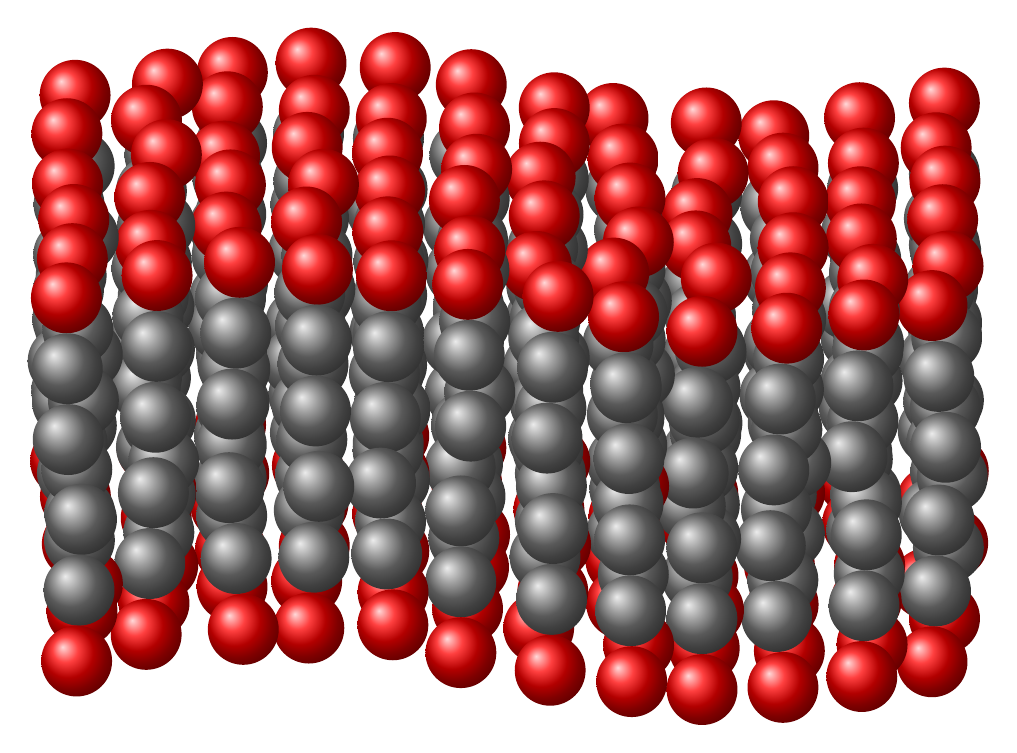
\begin{tikzpicture}
  \def\nuPi{3.1459265}
  \foreach \i in {11,10,...,0}{% This one doesn't matter
    \foreach \j in {5,4,...,0}{% This will crate a membrane
                               % with the front lipids visible
      % top layer
      \pgfmathsetmacro{\dx}{rand*0.1}% A random variance in the x coordinate
      \pgfmathsetmacro{\dy}{rand*0.1}% A random variance in the y coordinate,
                                     % gives a hight fill to the lipid
      \pgfmathsetmacro{\rot}{rand*0.1}% A random variance in the
                                      % molecule orientation      
      \shade[ball color=red] ({\i+\dx+\rot},{0.5*\j+\dy+0.4*sin(\i*\nuPi*10)}) circle(0.45);
      \shade[ball color=gray] (\i+\dx,{0.5*\j+\dy+0.4*sin(\i*\nuPi*10)-0.9}) circle(0.45);
      \shade[ball color=gray] (\i+\dx-\rot,{0.5*\j+\dy+0.4*sin(\i*\nuPi*10)-1.8}) circle(0.45);
      % bottom layer
      \pgfmathsetmacro{\dx}{rand*0.1}
      \pgfmathsetmacro{\dy}{rand*0.1}
      \pgfmathsetmacro{\rot}{rand*0.1}
      \shade[ball color=gray] (\i+\dx+\rot,{0.5*\j+\dy+0.4*sin(\i*\nuPi*10)-2.8}) circle(0.45);
      \shade[ball color=gray] (\i+\dx,{0.5*\j+\dy+0.4*sin(\i*\nuPi*10)-3.7}) circle(0.45);
      \shade[ball color=red] (\i+\dx-\rot,{0.5*\j+\dy+0.4*sin(\i*\nuPi*10)-4.6}) circle(0.45);
    }
  }
\end{tikzpicture}
\end{document}